\newcommand{\PRF}{\ensuremath{{\sf PRF}}}
\newcommand{\FHE}{\ensuremath{{\sf FHE}}}
\newcommand{\Gen}{\ensuremath{{\sf Gen}}}
\newcommand{\Eval}{\ensuremath{{\sf Eval}}}
\newcommand{\DpfGen}{\ensuremath{{\sf DPF.Gen}}}
\newcommand{\DpfEval}{\ensuremath{{\sf DPF.Eval}}}
\newcommand{\Enc}{\ensuremath{{\sf Enc}}}
\newcommand{\Dec}{\ensuremath{{\sf Dec}}}
\newcommand{\Dpf}{\ensuremath{{\sf DPF}}}
\newcommand{\DPF}{\ensuremath{{\sf DPF}}}
\newcommand{\Prg}{\ensuremath{{\sf PRG}}}
\newcommand{\Pbc}{\ensuremath{{\sf PBC}}}
\newcommand{\Seed}{\ensuremath{{\sf Seed}}}
\newcommand{\DB}{\ensuremath{{\sf DB}}}
\newcommand{\Comm}{\ensuremath{{\sf Comm}}}
\newcommand{\GenSched}{\ensuremath{{\sf GenSchedule}}}
\newcommand{\ServerPre}{\ensuremath{{\sf ServerPreprocess}}}
\newcommand{\ClientQ}{\ensuremath{{\sf ClientQuery}}}
\newcommand{\ServerA}{\ensuremath{{\sf ServerAnswer}}}
\newcommand{\ClientD}{\ensuremath{{\sf ClientDecode}}}
\newtheorem{notation}{Notation}
\newcommand{\xor}{\ensuremath{\oplus}}
\newcommand{\Sim}{\ensuremath{{\sf Sim}}}
\newcommand{\negl}{\ensuremath{{\sf negl}}}
\newcommand{\get}{\ensuremath{\leftarrow}}
\newcommand{\Client}{\textsf{Client}~}
\newcommand{\Server}{\textsf{Server}~}
\newcommand{\CV}{\ensuremath{{\sf CV}}}
\newcommand{\key}{\ensuremath{{\sf key}}}
\newcommand{\getr}{\ensuremath{~{\overset{\$}{\leftarrow}}}~}
\newcommand{\ignore}[1]{}

\section{Distributed Point Function and 2-server PIR with $O_{\lambda}(\log(n))$ Communication ~\cite{boyle2016function}}

We saw that in the IT-setting, the best known upper bound on the communication of 2-server PIR scheme is by Dvir and Gopi~\cite{dvir20162}.
The scheme achieves $n^{O(\sqrt{\log \log n / \log n})}$ communication.
In this lecture, we see that if we are willing to assume that one-way functions (OWF) exist, we can construct a 2-server PIR scheme with $O_\lambda(\log n)$ communication.

\subsection{Basic Idea}
This scheme use pseudorandom generators (PRG). In particular, PRG implies the existence of OWF and OWF implies the existence of PRG~\cite{haastad1999pseudorandom}. 

\begin{definition}[PRG]
    Let $l(\cdot)$ be a polynomial and G: $ \{0,1\}^n \rightarrow \{0,1\}^{l(n)}$ be a deterministic
    polynomial time algorithm. G is a \Prg \ if it has the following properties:
    \hfill
    \begin{itemize}
        \item \textbf{Expansion:} $\forall n, l(n) > n$.
        \item \textbf{Pseudorandomness:} $\forall$ PPT distinguishers D, $\exists$ negl() s.t.
        $$\left|\Pr[D(r) = 1] - \Pr[D(G(s)) = 1]\right| \leq negl(n)$$ 
        Where $r \overset{{\scriptscriptstyle\$}}{\leftarrow} \mathcal{U}^{l(n)}$ and
        $s \overset{{\scriptscriptstyle\$}}{\leftarrow} \mathcal{U}^{n}$.
    \end{itemize}
\end{definition}


\begin{notation}
    For $x \in\{0,1\}^*$, the point function $P_{x}:\{0,1\}^{|{x}|} \rightarrow \{0,1\}$
    is defined by $P_{x^*}(x^*) = 1 \ and \ P_{x^*}(x) = 0$ for all $x \neq x^*$.
\end{notation}

Boyle, Gilboa and Ishai~\cite{boyle2016function} introduced the concept of distributed point function. 
We are going to focus on the case of a 2-share binary distributed point function. 
Essentially, given the full description of the point function $P_{x^*}$, one can ``secretly share'' the function to two keys $k_0,k_1$. Then, if party $t\in\{0,1\}$ receives $k_t$, it can evaluate the key on all possible location $x$ and get an evaluation of $\Eval(k_t, x)$. 
It is guaranteed that in every location $x'$, $\Eval(k_0, x)\xor\Eval(k_1, x)=P_{x^*}(x)$.
Also, each party $t$ has no information about the ``special location'' (i.e., $x^*$) given the key $k_t$.


\begin{definition}[2-share binary \Dpf]
    A DPF is a pair of PPT algorithms (\Gen,\Eval) with the following syntax:
    \hfill
    \begin{itemize}
        \item $\Gen(1^\lambda,x^*)$: Outputs a pair of keys $k_0,k_1$.
        \item $\Eval(1^\lambda, k,x)$: Outputs $y \in \{0,1\}$
    \end{itemize}
    \paragraph{Correctness.} $\Pr[k_0,k_1 \leftarrow \Gen(1^\lambda, x^*):\Eval(k_0,x) \oplus \Eval(k_1,x) = P_{x^*}(x)] = 1$.
    \paragraph{Privacy.} Given $t\in\{0,1\}$ and any $x^*\in \{0,1\}^\ell$, there exists a PPT simulator $\Sim$, such that the following experiments are computaionally indistinguishable:
    \begin{itemize}
        \item $\mathsf{Real}(1^\lambda)$: $k_0,k_1\get  \Gen(1^\lambda, x^*)$ and output $k_t$;
        \item $\mathsf{Ideal}(1^\lambda)$: Output $\Sim(1^\lambda, \ell)$.
    \end{itemize}
\end{definition}


\subsection{2-server PIR scheme based on DPF}

Let $\DB \in \{0,1\}^{n}, i \in [n]$ and $\lambda$ be the security parameter.
Suppose we have an efficient 2-share binary DPF scheme $\DpfGen$ and $\DpfEval$, such that the key length is $O_\lambda(\log n)$ (where $n$ is the size of the input domain), and the evaluation algorithm is efficient. 
Then, we can have the following 2-server PIR scheme. %n the following, when the context is clear, we will omit $1^\lambda$ in the description.

\begin{enumerate}
    \item Given the query $i$, \Client computes $(k_0,k_1) \leftarrow \DPF.\Gen(1^\lambda, i)$
    \item \Client sends $(k_0,k_1)$ to \Server 0 and \Server 1 respectively.
    \item For $t\in\{0,1\}$, \Server $t$ responds with $y_i \leftarrow \bigoplus_{j\in [n]} \DPF.\Eval(k_t,j)\cdot \DB[j]$;
    \item \Client computes the answer as $y_0 \oplus y_1$.
\end{enumerate}

\paragraph{Correctness} 
\begin{align*} 
    y_0 \oplus y_1 & = \left(\bigoplus_{j}\DB[j]\cdot \DpfEval(k_0,j) \right) \oplus \left(\bigoplus_{j}\mathsf{DB}[j]\cdot \DPF.\Eval(k_1,j) \right) \\
    & = \left(\bigoplus_{j}\DB[j]\cdot (\DpfEval(k_0,j)\xor \DPF.\Eval(k_1,j)) \right) \\
    & = \left(\bigoplus_{j}\DB[j]\cdot P_{i}(j)\right) \\
    & = \DB[i].
\end{align*}
\paragraph{Security}
Security follows from the security of the DPF.



\subsubsection{DPF construction using PRG}



\begin{figure}
    
    \begin{minipage}{\textwidth}
        \begin{mdframed}
            \paragraph{Initialization:} 
            %Repeat the following process $m$ times (indexed by $j$):
            \begin{itemize}
                \item Sample $s_0$, $s_1$ as two random $\lambda$-bit random strings. 
                \item Sample a random bit $b_0$. Let $b_1=b_0\xor 1$.
                \item Let $k_0 = (s_0, b_0)$ and $k_1=(s_1,b_1)$;
                \item Let $\{x^*[1],\dots,x^*[\log n]\}$ be $x^*$'s binary representation. 
            \end{itemize}
            
            
            \paragraph{Constructing correction vectors:} 
            
            
            For $i\in \{1,\dots, \log n\}$: 
            \begin{itemize}
                \item Let $s^0_L || b^0_L || s^0_R || b^0_R\get G(s_0)$;
                \item Let $s^1_L || b^1_L || s^1_R || b^1_R\get G(s_1)$;
                \item Let $s^*_L || b^*_L || s^*_R || b^*_R=(s^0_L || b^0_L || s^0_R || b^0_R) \xor (s^1_L || b^1_L || s^1_R || b^1_R)$;
                \item Sample $r$ as a random $\lambda$-bit random string;
                \item If $x^*[i]=0$: let $\CV_i =~ r ~|| b^*_L \xor 1 || s^*_R || b^*_R$;\hfill \textit{If the path goes left;} 
                \item If $x^*[i]=1$: let $\CV_i = s^*_L || b^*_L || ~r ~|| b^*_R \xor 1$;\hfill \textit{If the path goes right}; 
                
                \item Expand $(s_0, b_0), (s_1, b_1)$ to their children as the same as the expansion algorithm, using $\CV_i$. Update $(s_0, b_0), (s_1, b_1)$ by replacing them with their children's pairs (only the pairs on the special path).  
            \end{itemize}
            
            \paragraph{Output}:
            \begin{itemize}
                \item Attach $\CV_1,\dots,\CV_{\log n}$ to $k_0$ and $k_1$.
                \item Output $k_0,k_1$.
            \end{itemize}
            
        \end{mdframed}
    \end{minipage}
    \caption{The 2-share binary DPF generation algorithm.\label{fig:DPF}}
    %\caption{Detailed description of \name.\label{fig:single-server}}
\end{figure}

\begin{figure*}
    \centering
    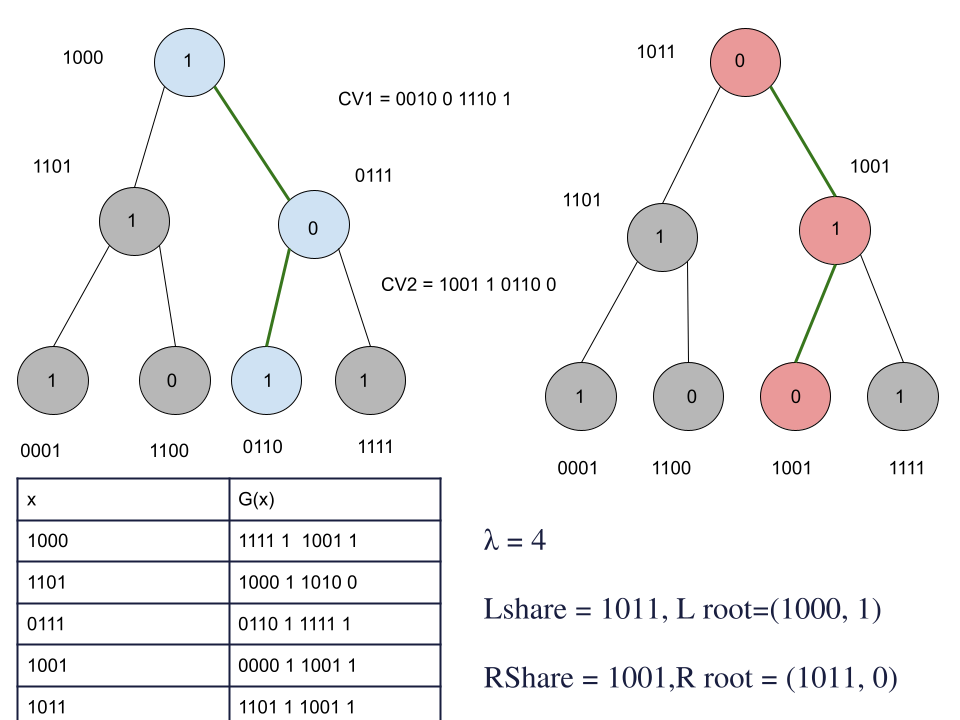
\includegraphics[scale=0.4]{scribimg_dpftree.png}
    \caption{An example of the DPF construction.\label{fig:example-DPF}}
\end{figure*}


Now we see how to construct this efficient 2-share binary DPF, based on a \Prg \ G:
 $$G: \{0,1\}^{\lambda} \rightarrow  \{0,1\}^{2\lambda + 2}. $$
The algorithm is based on a binary tree expansion.
%Where the series of evaluation results can be visualized as a binary tree.
 
\paragraph{The key structure.} The $\Gen$ algorithm outputs two keys, $k_0, k_1$. For each key $\key_t$ where $t\in\{0,1\}$, it contains the ``root'' information as a $\lambda$-bit random string $s$ and a bit $b\in\{0,1\}$. It also contains $\log n$ ``correction vectors'' $\CV_1, \dots, \CV_{\log n}$, each of size $2\lambda+2$ bit. $k_0, k_1$ will share the same sets of correction vectors. 
We will see how they are constructed later. 


\paragraph{Evaluation algorithm.} 
Given a key containing $s,b$ and $\CV_1,\dots,\CV_{\log n}$, the evaluation algorithm is as follows.
We consider a binary tree with $\log n + 1$ levels and $n$ leaves (assume $n$ is a power of 2). 
The root is on the $0$-th level and the leaves are on the $\log n$-th level.
Each node contains a key $ s \in \{0,1\}^{\lambda}$ (a $\lambda$-bit random string) and a bit $b \in \{0,1\}$. 
Suppose now we want to expand the information of this node (on level $i-1$) to its two children (on levle $i$), we only need the following one-line expansion algorithm:
 $$ s_{L} || b_{L} || s_{R} || b_{R} \leftarrow G(s) \oplus
 \begin{cases} 
    0 & b = 0; \\
    \CV_i & b = 1. \\
 \end{cases}$$
That is, $s_{L}, b_{L}$ are the information on its left child, and $s_{R}, b_{R}$ are the information on its right child.
Finally, the bit on the $i$-th leaf will be $\Eval(\key, i)$.

Notice that if we only want to learn $\Eval(\key, i)$ for a particular $i$, the computation cost will be $O(\log n)$ calls to the PRG, because we can focus on the path from the $i$-th leaf to the root and ignore other nodes.
%And on the path we only do $\log n$ expansions.
However, if we want to learn $\Eval(k, i)$ for all $i\in[n]$, the computation cost will be $O(n)$ because we can simply do the expansion on the whole tree. 


\paragraph{Generation Algorithm.} The generation algorithm needs to generate two correlated keys, such that when we look at the bit at the $x$-th leaves (say $b^0_{x}$ and $b^1_{x}$) on the trees expnaded by $k_0$ and $k_1$, it must that $b^0_{x}\xor b^1_{x}=P_{x^*}(x)$. In fact, we want to ensure the following stronger properties.
Say on a particular node, we denote the information expanded by $k_0$ and $k_1$ as $(s_0,b_0)$ and $(s_1,b_1)$, respectively.
\begin{enumerate}
    \item If the node is on the ``special path'' (i.e., the path from the root to the $x^*$-th leaf), then $b_0\ne b_1$, and $s_0$ and $s_1$ are independent.
    
    \item Otherwise, $b_0=b_1$ and $s_0=s_1$.
\end{enumerate}

The properties hold for the leaf nodes, which is sufficient to prove the correctness of the DPF.
We now see the how do we ensure these properties.
We have the first lemma, which can be proved by a simple induction argument.

\begin{lemma}
    If on some particular node, $b_0=b_1$ and $s_0=s_1$, then the subtrees expanded based on $(s_0,b_0)$ and $(s_1,b_1)$ will be identical, regardless of $CV_1,\dots,CV_{\log n}$.
\end{lemma}

This lemma shows that we only need to focus on the ``special path''. We can sample the root information first by sampling two random strings $s_0,s_1$ and let $b_0$ and $b_1$ be two different bits. 
Then, we can just ``simulate'' the expansion process on the special path, and then set up the correction vector according to the target properties. 
Since on the $i$-th level of the special path, there will be only one side affected by the correction vector (because the bits are different).
Therefore, we can always set the correction vector to ensure that after applying the correction vector, the children on the special path still have different bits and independent random strings, while the children deviating from the path will become identical.
The algorithm is presented in Figure~\ref{fig:DPF} and an example is presented in Figure~\ref{fig:example-DPF}.


\paragraph{Analysis.}
The correctness can be verified by doing an induction proof from level $1$ to level $\log n$.
The privacy analysis is referred to~\cite{boyle2016function}. 
It is also clear to see that the key size is $\lambda+1+\log n\cdot (2\lambda+2)=O_\lambda(\log n)$.



 \section{Batch-PIR}

 \subsection{Motivation}
    So far, every PIR scheme we have seen only retrieves 1 bit at a time. This works great for yes/no questions,
    but is cumbersome if we wanted to do anything practical. For instance, to compute Q queries using a naive PIR scheme with $O(n)$ computation, it requires $O(Qn)$ computation.
    Batch-PIR aims to make PIR more practical by enabling multiple
    responses for a single query, grouping together multiple responses into one and reduce the
     amortized cost.
     
     
\subsection{A simple load-balancing scheme}

Given an $n$ bit long database and $Q=o(n)$ queries, we load-balance the database into $\frac{Q}{\log Q}$ buckets -- we use a hash function to hash each database entry to a bucket and place it there.
Then, given the $Q$ queries, we again use the hash function to place the queries to the buckets. 
In expectation, each bucket will have $\log Q$ queries. 
Based on the balls-into-bins argument, each bucket will have no more than $\lambda \log Q$ queries with $1-\negl(\lambda)$ probability.
Therefore, we just do $\lambda \log Q$ PIR queries in each bucket (possibly dummy queries) to retrieve the target entries. 
This ensures the success probability is at least $1-\negl(\lambda)$.

\paragraph{Security.}
We are always making fix number of queries ($\lambda \log Q$ PIR queries in each bucket), so the scheme is secure by a reduction to the security of the underlying PIR scheme.

\paragraph{Cost.}
Moreover, say the underlying single-query PIR computation cost is linear in the size of the database.
We are making $\lambda \log Q$ queries to each bucket, and the total size of the buckets is just $n$. 
Therefore, the total computation cost is $O(\lambda \log Q n)$. 
So if $Q>\lambda \log Q$, this simple scheme saves computation.


     
     
\subsection{Cuckoo Hashing based scheme~\cite{angel2018pir}}

Angel et al.~\cite{angel2018pir} proposed SealPIR that uses cuckoo hashing to do batch PIR.
    
    \paragraph{Cuckoo Hashing}
    \begin{definition}[Cuckoo hashing]
        Given $n$ balls, $b$ buckets, and $w$
independent hash functions $h_0$, $\cdots$ , $h_{w}$ that map a ball to a
random bucket, compute $w$ candidate buckets for each ball by
applying the $w$ hash functions. For each ball $x$, place $x$ in any
empty candidate bucket. If none of the $w$ candidate buckets
are empty, select one at random, remove the ball currently in
that bucket ($x_{\text{old}}$), place $x$ in the bucket, and re-insert $x_{\text{old}}$. If
re-inserting $x_{\text{old}}$ causes another ball to be removed, this process
continues recursively until we finish the insertion or a maximum number of iterations is achieved.
    \end{definition} \
    
\paragraph{Batch PIR based on Cuckoo Hashing.}   
The scheme is as follows.
\begin{itemize}
    \item \textbf{Serer encoding.} Given an $n$ bit database, $b$ buckets, and $w$ hash functions, we hash each entry in the database (using their index as the key) to all $w$ candidate buckets and store it there.
    This results in a encoded database that each original entry is replicated $w$ times.
    The server will share the hash functions to the client.
    
    \item \textbf{Client scheduling.} Given the $Q$ queries, the client use the cuckoo hashing method to insert (or say, schedule) the queries to the buckets (again, using the indices as the keys).
    Our target is that each bucket has at most one query, and all query can be inserted in one of its candidate bucket.
    
    \item \textbf{Client query.}. Now the client just makes one query in each bucket. If the client successfully insert all queries earlier, it can then proceed to learn all the target entries because the server has inserted the entries in all the candidate buckets.
\end{itemize}

An example can be found in Figure~\ref{fig:sealpir}.
   
The authors used 3 hash functions for encoding and set the number of buckets $b = 1.5Q$. For $Q\geq 200$, the author showed that the chance of failure during
the scheduling phase is $\leq 2^{-40}$.
Notice that this is not cryptographically neligible. 
To enforce negligible failure probability, we can introduce a size $\lambda$ stash of the cuckoo hash table.
That is, the stash stores at most $\lambda$ elements that fail to be inserted. 
Then, the client also has to make additional $\lambda$ PIR queries to the whole database.
This ensures the failure probability to be $\negl(\lambda)$.

\paragraph{Cost Analysis.} 
Assume the underlying single-query PIR scheme is linear.
The client will make one query in each bucket and the total bucket size is $wn$.
Also, the client needs to make $\lambda$ additional query to the whole database to ensure negligible failure probability.
Then, the computation cost for the $Q$ queries are just $(w+\lambda)n$.

    
    
\begin{figure*}
    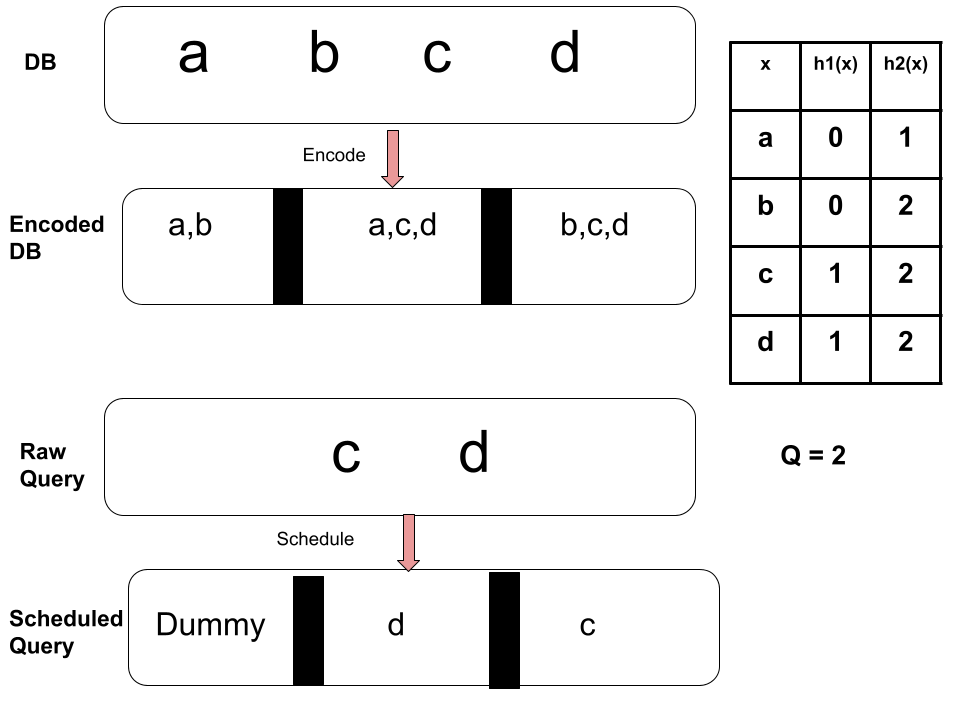
\includegraphics[scale=0.45]{scribimg_batchpir.png}
    \caption{An example of the cuckoo hashing based batch PIR. \label{fig:sealpir}}
\end{figure*}












\ignore{

%%%%%%%%%%%%%

Intuitively, this just applies all hash functions to an entry. If all buckets it gets hashed to are
taken, it will choose a random bucket, remove the ball currently in there and re-insert
using the same procedure. \\
\paragraph{Probabilistic Batch Codes}
\begin{definition}[Batch Code ~\cite{angel2018pir}]
    A (n, m, k, b)-batch code B takes as input a collection DB of n
    elements, and produces a set of m codewords, C, distributed
    among b buckets. Formally, $B : DB \rightarrow (C_0,..., C_{b})$, where
    $|Ci|$ is the number of codewords in bucket i, and the sum of
    codewords across all buckets is $m = \sum_{i=0}^{b-1}|Ci| \geq n$.
    The goal of these codes is two-fold. First, they ensure that any k elements
    from DB can be retrieved from the b buckets by fetching at most
    one codeword from each bucket. Second, they keep the number
    of total codewords, m, lower than $k \cdot n$.
\end{definition}
Batch codes incur a large network overhead by guaranteeing completeness in that it
is always possible to retrive k codewords by querying k distinct buckets. By adding possibility of failure p,
bandwidth can be shaved off at the cost of a chance of query failure. Applying this relaxation
results in a Probabilistic Batch Code, which is how SealPIR is able to encode a database
into multiple sub-databases that can be queried simultaneously with PIR. Informally, they are defined by 3 functions:
\begin{itemize}
    \item \textbf{\sf Encode(DB):} Split the database and replicate entries accordingly.
    \item \textbf{\sf GenSchedule(W):} Generate a query to each subdatabase such that all desired items are retrieved.
    \item \textbf{\sf Decode(I):} Extracts individual responses from the server response.
\end{itemize}
A formal definition and construction using reverse hashing can be found on page 6 of ~\cite{angel2018pir}


\subsection{The SealPIR scheme}

\paragraph{Intuition} The main idea is to build a \Pbc \ over the PIR database. The only major modifications
are to GenSchedule and Decode, where the equeries must be modified to be PIR queries. While failures in the query scheduling phase are
possible, the authors tune the parameters to make the likelihood very low.
\\
\paragraph{Notation}
Let \Pbc = $(\mathsf{Encode},\GenSched,\mathsf{Decode})$ be a Probabilistic Batch code constructed using Cuckoo hashing. Additionally,
Let PIR = (\ServerPre,\ClientQ,\ServerA,\ClientD) be a PIR scheme.

\paragraph{\sf SealPIRPreprocess} Given w independent hash functions $H = (h_1,...,h_w)$ and \DB, output b buckets $B = {B_1,...,B_b}$, where:
$$\sf B_i = SealPIRPreprocess(s_i),(s_0,...s_b) = encode(DB) $$
\paragraph{\sf SealPIRQuery} For a set of Q queries $q_1,...,q_b$, and Cuckoo hashing algorithm CK:
\begin{enumerate}
    \item Client computes $\sigma \leftarrow GenSchedule(Q)$
    \item if $\sigma \neq \perp$ goto (3) else  return failure
    \item Client computes $(q_1,...q_b) \leftarrow (ClientQuery(B_0,\sigma[0]),...,ClientQuery(B_Q,\sigma[b]))$ and sends the result to the server
\end{enumerate}
Where $\sigma \in \{\{1,....,b\}\}^b$ maps queries to the bucket the query should go to. $\sigma == \perp$ if there were two indices mapped to the same bucket.

\paragraph{\sf SealPIRAnswer} Server computes and sends $$r_i = \ServerA(B_i,\sigma[i]), \forall i \in [Q]$$ back to client.
\paragraph{\sf SealPIRDecode} To retreive the answer to the ith query, the client computes:
$$a_i \leftarrow \sf Decode(ClientDecode(r_i))$$

%%%%%%%%%%%%%



}
